\documentclass[11pt]{article}
\usepackage{fullpage,amsthm,amsfonts,amssymb,epsfig,amsmath,times,amsthm}
\usepackage{tabu} 
\usepackage{pgfplots}

\newtheorem{theorem}{Theorem}
\newtheorem{claim}[theorem]{Claim}
\newcommand\tab{\setlength\parindent{24pt}}

\begin{document}
	
	\begin{center}
		{\bf\Large CMPS 102 --- Fall 2018 --  Homework 3}\\
		Alyssa Melton\\
		I have read and agree to the collaboration policy. \\
		Collaborators: none\\
	\end{center}
	
	%------------------------------------------------------------------------------	
	%------------------------------------------------------------------------------
	
	\section*{Solution to Problem 1}
		We are given a set of days, 1 to \textit{n}. 
		For each corresponding day, we are given the price of the crop. 
		We want to find the maximum amount of profit that Phillip could have made in these \textit{n} days.
		
		While thinking through different things that might help to solve this problem, I graphed prices of crop over \textit{n} days that were given as an example, namely: \\
		\\
		\begin{tabu} to 1 \textwidth { | X[c] | X[c] | X[c] | X[c] | X[c] | X[c] | X[c] | X[c] | X[c] | X[c] | X[c] | X[c] | X[c] | X[c] | X[c] |}
			\hline
			Day & 1 & 2 & 3 & 4 & 5 & 6 & 7 & 8 & 9 & 10 & 11 & 12 & 13 & 14 \\
			\hline
			Price  & 13  & 11 & 8 & 10 & 7 & 12 & 12 & 17 & 14 & 9 & 6 & 8 & 12 & 11  \\
			\hline
		\end{tabu}\\
	\\
	\\
		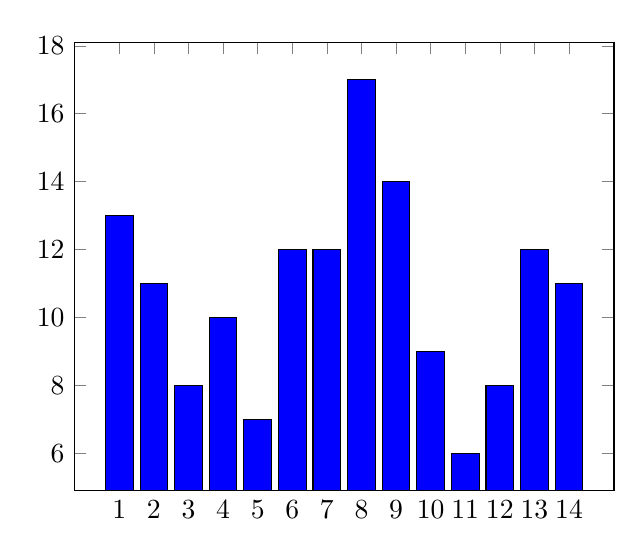
\begin{tikzpicture}
				\begin{axis}[
				symbolic x coords={1, 2, 3, 4, 5, 6, 7, 8, 9, 10, 11, 12, 13, 14},
				xtick=data
				]
				\addplot[ybar,fill=blue] coordinates {
					(1,   13)
					(2,  11)
					(3,   8)
					(4, 10)
					(5, 7)
					(6, 12)
					(7, 12)
					(8, 17)
					(9, 14)
					(10, 9)
					(11, 6)
					(12, 8)
					(13, 12)
					(14, 11)

				};
				\end{axis}
		\end{tikzpicture} \\
		\\
		We are given that the most profit is gained, for this particular example, is by doing the following:\\
		Buy a cart on day 3, sell the cart on day 4, with a margin of 2;\\
		buy a cart on day 5, sell a cart on day 8, with a margin of 10;\\
		buy a cart on day 11, sell a cart on day 13, with a margin of 6.\\
		Now, comparing these values to the graph above, I noticed that these directly correspond with the peaks and valleys of the graph. \\
		\\
		Defintions:\\
		A day's crop price, $price[x]$, is a peak if $price[x] \leq price[x-1]$ and $price[x] \geq A[x+1]$\\
		A day's crop price, $price[x]$, is a valley if $price[x] \geq price[x-1]$ and $price[x] \leq A[x+1]$\\
		\\
		Let us assume that the most profit is gained by buying crop at a price valley, and selling crop at a price peak. Now, consider the following algorithm:\\
		\\
		$profit = 0.\\
		purchase price = null.\\
		profit margin = null.
		price[0] = null.\\
		price[n+1] = null$.\\
		\\
		for each day \textit{i}, 1 to \textit{n}:\\
		\indent  if $price[i-1] \geq price[i]$ and $price[i] \leq price[i+1]$\\
		\indent \indent if $purchase price = null$\\
		\indent \indent \indent buy crop on day \textit{i}.\\
		\indent \indent \indent purchase price = $price[i]$\\
		\indent else if $price[i-1] \leq price[i]$ and $price[i] \geq price[i+1]$\\
		\indent \indent if $purchase price \neq null$ \\
		\indent \indent \indent sell crop on day \textit{i} \\
		\indent \indent \indent $profit margin = price[i] - purchase price$ \\
		\indent \indent \indent $profit = profit + profit margin$ \\
		return \textit{profit}.
		

	\begin{claim} 
		The most profit is gained by buying crop at a price valley, and selling crop at a price peak. (The algorithm is optimal)
	\end{claim}

	\begin{proof}
			Assume that the most profit is not gained by buying crop at a price valley and selling crop at a price peak. Then there must be some other algorithm call it \textit{B} that is optimal. Say that \textit{B} and \textit{A} are the same up until day \textit{k}, where \textit{B} either buys or sells at a time that \textit{A} does not.\\
			\\
			Case 1: At day \textit{k}, \textit{B} buys at a time that is not a valley. 
			
				Call the day which is a valley that \textit{A} buys on $j$. Then by definition of a valley, $j$ is necessarily cheaper/less expensive than $k$. Then, no matter where in the future \textit{B} sells, be it the highest priced day after that buy, call it $h$, $(price(h) - price(j)) > (price(h) - price(k))$, since $k > j$. Thus, \textit{O} made no more profit than \textit{A}. \\
			\\
			Case2: At day \textit{k}, \textit{O} sells at a time that is not a peak.
				
				Call the day which is a peak that \textit{A} sells on $j$. Then by definition of a peak, $j$ is necessarily more valuable/more expensive than $k$. Then, no matter where in the past \textit{B} bought, be it the lowest priced day before that buy, call it $h$, $(price(j) - price(h)) > (price(k) - price(h))$, since $j > k$. Thus, \textit{O} made no more profit than \textit{A}. \\
				
	\end{proof}

	\begin{claim} 
	The above algorithm is $O(n)$. 
\end{claim}

\begin{proof}
	For each day, 1 to \textit{n} we are doing two comparisons, and either buying, selling, or doing nothing. If we call each comparison +1 and each buy or sell +1, then we are doing at most $3$ operations every day, for $n$ days. This is at most $3n$ operations, which is $O(n)$.
\end{proof}

	\newpage
	
	
\end{document}
